\documentclass[main.tex]{subfiles}
\begin{document}

\chapter{Energy reconstruction}
\label{chap:energy_reconstruction}
\label{chapter:reconstruction}

This chapter describes the reconstruction chain that connects the station-level measurements of an event to an estimate of the primary cosmic-ray energy.
In \cref{sec:reconstruction_shower_size}, the \Offline reconstruction is used to determine the shower geometry and to estimate the signal at a reference distance from the shower axis through a fit of the \gls{ldf}.
The zenith-angle dependence caused by atmospheric attenuation is then determined and compensated in \cref{sec:cic}.
Finally, in \cref{sec:calibration}, the corrected shower size is calibrated against the energy estimator of the \sd{750} to assign an energy to each \sd{433} event.

\section{Reconstruction of the shower size}
\label{sec:reconstruction_shower_size}

The shower reconstruction proceeds in two stages.
First, the relative start times of the signals measured by the participating stations are used to determine the arrival direction of the shower.
The recorded signals are then fitted as a function of the perpendicular distance to the shower axis using an empirical \gls{ldf} to model the decrease in the signal with the distance to the core.
Analogously to the other \gls{sd} arrays, the value of this function at the reference distance of \SI{300}{\m}, denoted by $S(300)$, provides the ground-level shower-size estimator used for the \sd{433}~\cite{Silli:2021:PerformanceSD433}.
% Because the core position affects the station distances entering the \gls{ldf}, the geometry and shower size are finally determined in a combined fit initialized with the results of the separate reconstructions.
A detailed description of the event-reconstruction procedure used for the surface detector can be found in Ref.~\cite{PierreAuger:2020:SDReconstruction}.
Here, the main elements relevant to the reconstruction of the \sd{433} events are summarized, with particular emphasis on the steps implemented for the present analysis.

\subsection{Geometrical reconstruction}
\label{subsec:geometry_ldf}

The geometrical reconstruction uses the positions and signal start times of the detectors participating in the event.
Its purpose is to determine the unit vector along the shower axis, $\hat{a}$, whose components are the direction cosines from which the zenith angle, $\theta$, and the azimuth angle, $\phi$, are obtained. 

The reconstruction begins with a plane-front fit to the station start times, which provides an initial estimate of the arrival direction.
The signal-weighted barycentre of the participating stations is used as the initial estimate of the core position.
These estimates are subsequently refined using a curved description of the shower front.

In the \Offline reconstruction, the leading particles of the shower, which define the extreme shower front, are approximated by a sphere expanding at the speed of light from a virtual origin $\vec{x}_0$ at time $t_0$.
The predicted time at which this front reaches a position $\vec{x}$ is
\begin{align}
    c\,t_\mathrm{sh}(\vec{x}) = c\,t_0 + \lvert \vec{x}-\vec{x}_0 \rvert .
    \label{eq:spherical_shower_front}
\end{align}
The fit minimizes the squared differences between the measured and predicted start times,
\begin{align}
    \chi^2 = \sum_i \frac{\left[t_i-t_\mathrm{sh}(\vec{x}_i)\right]^2}{\sigma_{t_i}^2}.
    \label{eq:geometry_chi2}
\end{align}
where $t_i$ and $\sigma_{t_i}$ are the start time measured by station $i$ and its uncertainty, respectively.

% The core position is refined together with the lateral distribution of the station signals.
Once core position is determined, the reconstructed shower direction is given by
\begin{align}
    \hat{a}
    =
    \frac{\vec{x}_{0}-\vec{x}_{\mathrm{c}}}
    {\left|\vec{x}_{0}-\vec{x}_{\mathrm{c}}\right|}.
    \label{eq:shower_axis}
\end{align}
\noindent with the radius of curvature given by $R_{0}=\left|\vec{x}_{0}-\vec{x}_{\mathrm{c}}\right|$.

For events with at least five participating stations, the radius of curvature is determined from the timing fit.
For events with lower station multiplicity, the number of degrees of freedom is insufficient to constrain the curvature, and $R_{0}$ is fixed according to a parametrization obtained from higher-multiplicity events.

The left panel of \cref{fig:sd433_event_footprint_ldf} illustrates the geometrical reconstruction of an \sd{433} event.
The marker size is proportional to the station signal, while the colour scale represents its start time, progressing from earlier signals in blue to later signals in green.
The black line indicates the reconstructed arrival direction projected onto the ground, and the cross marks the reconstructed core position.

\subsection{Lateral distribution function}
\label{subsec:ldf}

The shower size is then estimated by modeling the fall-off of the signal $S(r)$ with the distance $r$ to the shower axis using a \gls{ldf} ~\cite{Silli:2021:PerformanceSD433}.
Intrinsic shower-to-shower fluctuations produce variations in the longitudinal development, such that individual events may be sampled at different stages of their development.
As a consequence, the \gls{ldf} slope exhibits variations on an event-by-event basis. 
Instead, the reconstruction is based on an \textit{average} LDF slope, $\langle S(r)\rangle$, and the expected signal at a fixed reference distance, $r_\text{opt}$, is adopted as the shower size.
The optimal distance of \qty{300}{m} for the \sd{433} is determined by fitting the LDF and identifying the distance at which the reconstructed shower size is minimally dependent on the assumed LDF slope, following the method described in Ref.~\cite{Newton:2007:OptimalDistance}.
The dependence of the optimal distance on the assumed LDF shape, the primary energy, and the zenith angle remains at approximately the 5\% level~\cite{PierreAuger:2020:SDReconstruction}.
The LDF is described using an empirically-chosen model based on a modified \gls{nkg} function,
\begin{align}
  \langle S(r)\rangle =
    S(r_\text{opt})
    \left(\frac{r}{r_\text{opt}}\right)^\beta
    \left(\frac{r + r_\text{scale}}{r_\text{opt} + r_\text{scale}}\right)^\beta,
\end{align}
%
\noindent where $\beta$ is the LDF slope and $r_\text{scale}=700\,\text{m}$ is a scale parameter.

The slope of the \gls{ldf} was determined on an event-by-event basis using a set of high-quality events with at least five triggered stations, for which $\beta$ could be left as a free parameter in the fit~\cite{Silli:2021:PerformanceSD433}.
The fitted values were then used to parametrize the average dependence of the slope on the shower size and zenith angle as
\begin{align}
    \beta(\theta,y)=a(\theta)+b(\theta) \, y,
\end{align}
\noindent where $y=\lg[S(300)/\text{VEM}]$.
The coefficients that govern the dependence on the zenith angle, $a(\theta)$ and $b(\theta)$ are modeled as second degree polynomials in $\sec\theta$,
\begin{align}
    \begin{pmatrix}
        a \\
        b
    \end{pmatrix}
    =
    \begin{pmatrix}
        -3.72 & 1.30  & 0.055 \\
         0.98 & -1.30 & 0.385
    \end{pmatrix}
    \begin{pmatrix}
        1 \\
        \sec\theta \\
        \sec^{2}\theta
    \end{pmatrix}.
    \label{eq:beta_parameterization}
\end{align}

The parameterization describes the slopes fitted for individual events with an average with a deviation of about $2\%$ over the considered range of shower sizes and zenith angles~\cite{Silli:2021:PerformanceSD433}.
Once determined, this parameterization was fixed in the reconstruction of the complete data set to determine the shower size $S(300)$ and the core position $\vec{x}_{\mathrm{c}}$ simultaneously through a maximum-likelihood fit.
The likelihood accounts for the measured signals in the triggered stations and for active stations that did not trigger.
Although no signal trace is available for these non-triggered stations, their presence constrains the fit, disfavoring an LDF predicting a signal above the trigger threshold at their positions.
In this way, the LDF fit determines $S(300)$ and refines the core position obtained from the initial geometrical reconstruction.

\begin{figure}
    \centering
    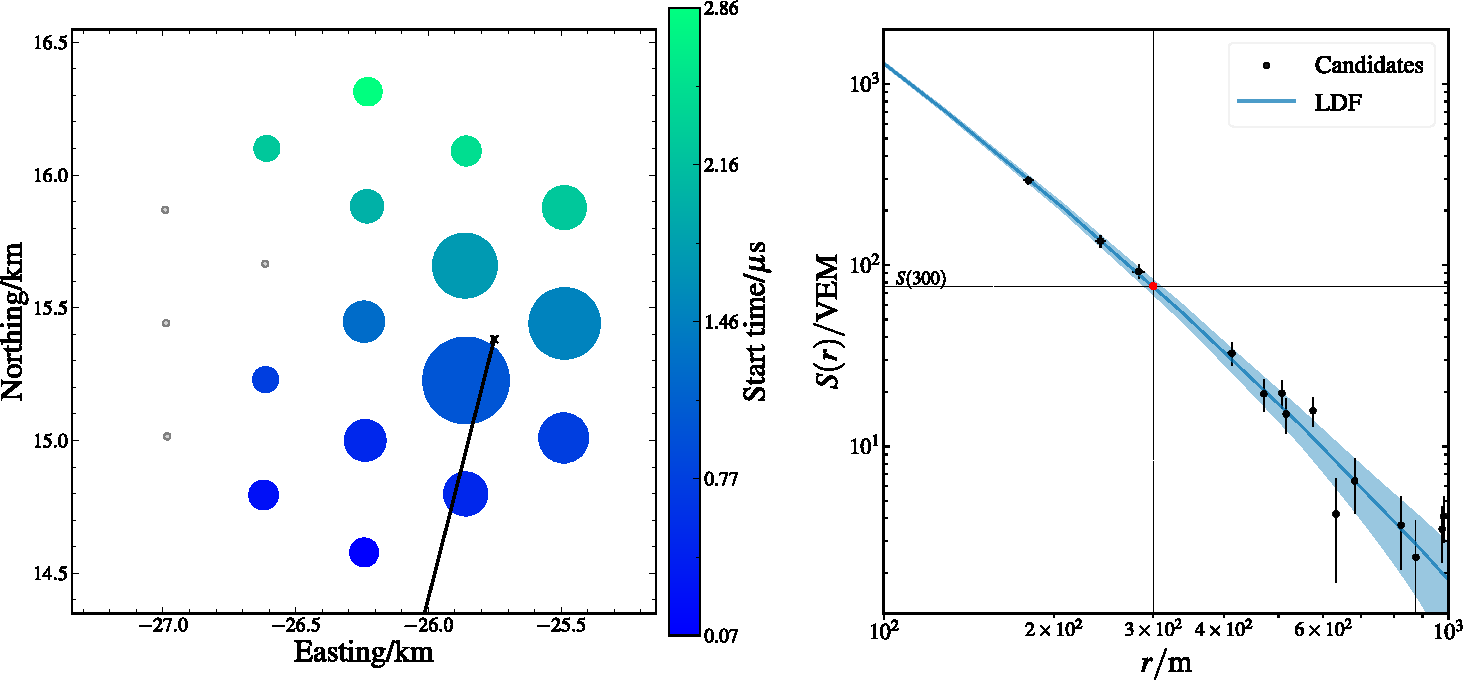
\includegraphics[width=\textwidth]{figures/chapter_reconstruction/event_footprint_ldf.pdf}
    \caption{Example reconstruction of an \sd{433} event with zenith angle $\theta=\ang{32.0}$ and reconstructed shower size $S(300)=\qty{76.5\pm2.9}{VEM}$. The left panel shows the event footprint and the right panel shows the recorded station signals as a function of the distance from the shower axis, together with the fitted \gls{ldf}. The red point indicates the reconstructed shower-size estimator $S(300)$. Other details are explained in the text.}
    \label{fig:sd433_event_footprint_ldf}
\end{figure}

The left panel of \cref{fig:sd433_size_zenith_distributions} shows the distribution of the reconstructed shower size.
At low values of $S(300)$, the number of events is strongly suppressed by the trigger efficiency.
It increases as the array approaches full efficiency and then the distribution decreases approximately as a power law, reflecting the steeply falling cosmic-ray flux.
The right panel shows the zenith angle distribution for the reconstructed events from 0 to $60^\circ$, the maximum angle of the vertical reconstruction implemented in \Offline.
The distributions contain \SDFourThreeTreeTotalNumberOfEvents\: reconstructed events.
However, as discussed in \cref{sec:efficiency}, only events with $\theta<40^\circ$ are used in the spectrum in order to lower the full efficiency threshold for the array.

In \cref{fig:sd433_multiplicity} the event multiplicity is shown in two $S(300)$ intervals, below and above $\qty{15}{VEM}$.
This threshold is chosen to roughly correspond to the signal of the full efficiency threshold.
For the lower $S(300)$ interval, most events have a low multiplicity of triggered stations.
For the higher $S(300)$ interval, which roughly corresponds to the data set used for the spectrum, $98\%$ of the events have a multiplicity greater than five.
This high multiplicity improves the quality of the reconstructed events and provides a robust measurement of the signal and the energy of the events.
\begin{figure}
    \centering
    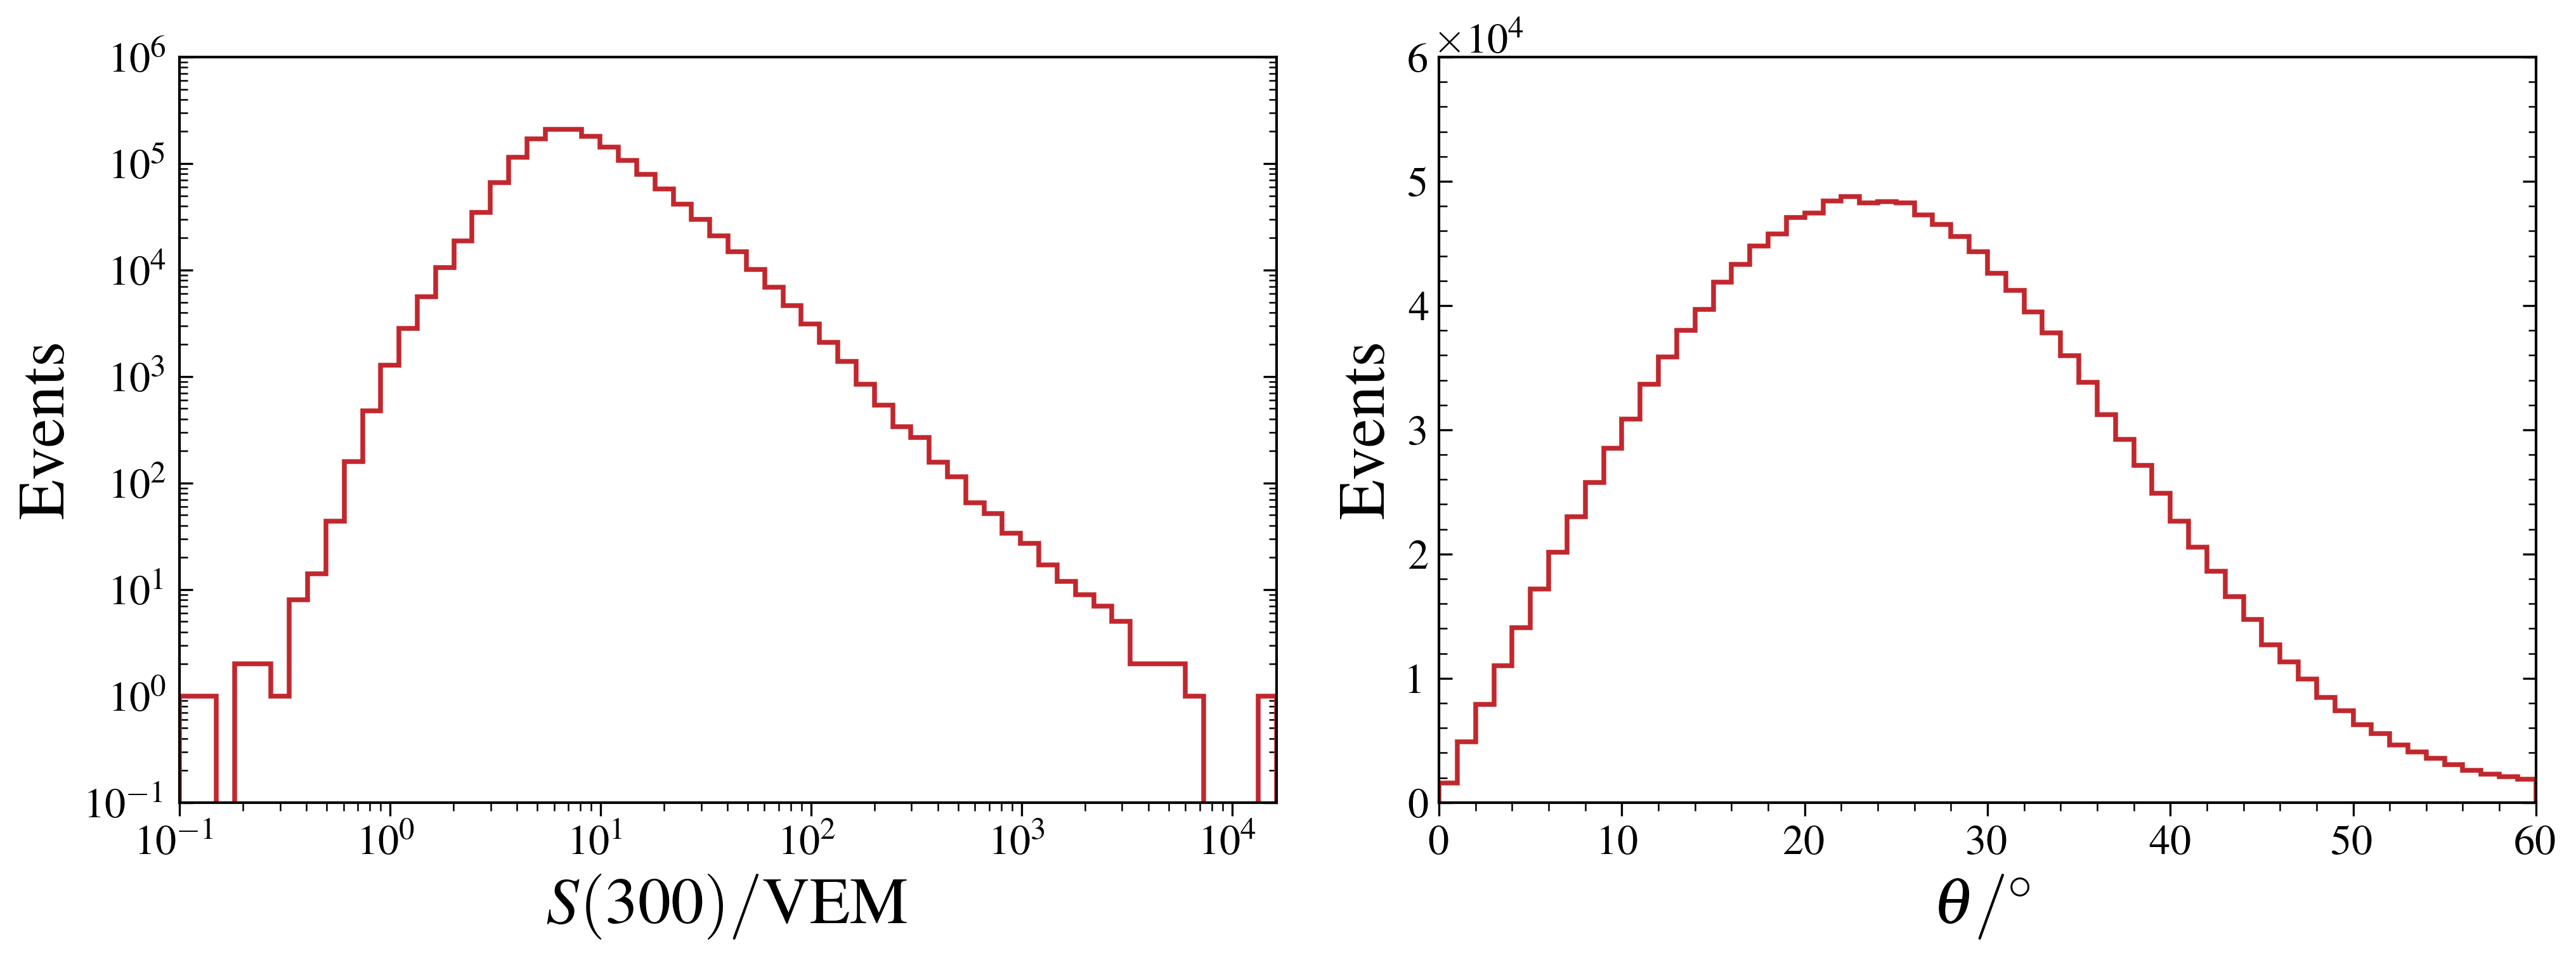
\includegraphics[width=\textwidth]{figures/chapter_reconstruction/shower_size_zenith_distributions.png}
    \caption{Distributions of the reconstructed shower size $S(300)$ (left) and zenith angle (right) for SD-433 events satisfying the 6T5 condition, with $0^\circ\leq\theta<60^\circ$.}
    \label{fig:sd433_size_zenith_distributions}
\end{figure}

\begin{figure}
    \centering
    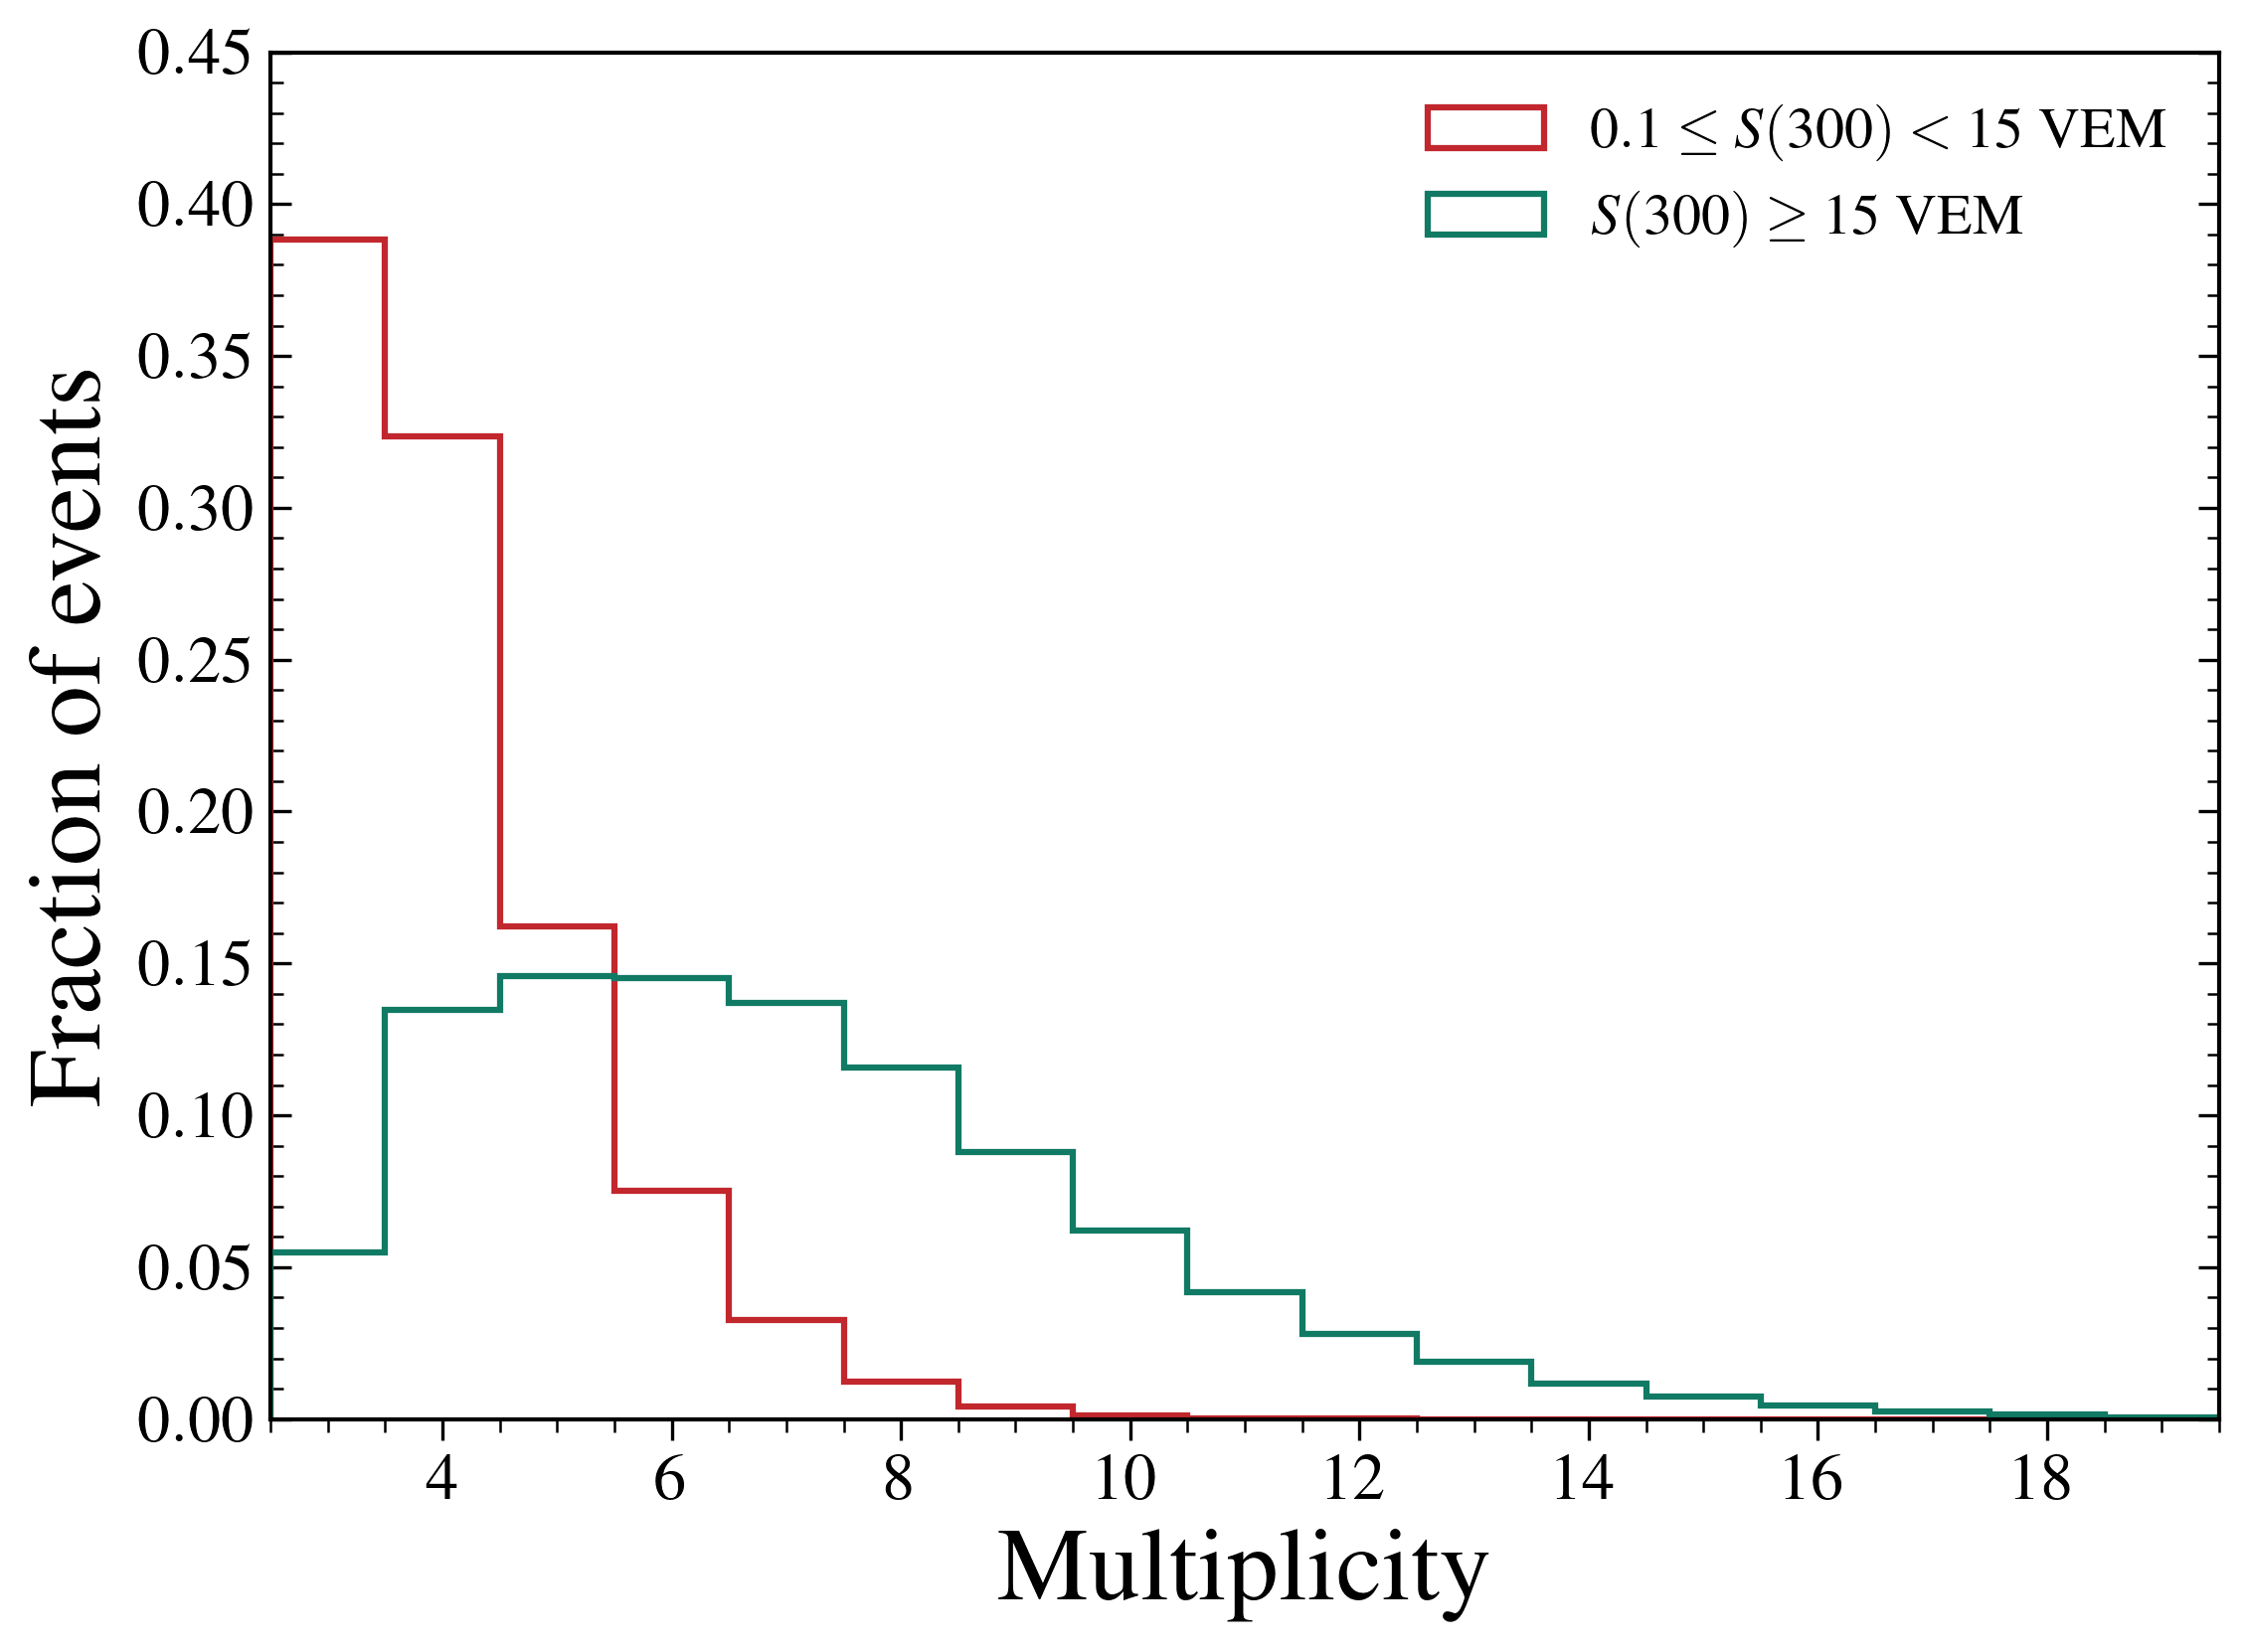
\includegraphics[width=0.78\textwidth]{figures/chapter_reconstruction/multiplicity_by_shower_size.png}
    \caption{Multiplicity of reconstructed events below and above $S(300)=15\,\mathrm{VEM}$. Each distribution is normalized independently to show the change in its shape with shower size.}
    \label{fig:sd433_multiplicity}
\end{figure}

\section{Correction for zenith-angle attenuation}
\label{sec:cic}

The reconstructed signal $S(300)$ provides an estimator of the shower size containing information about the energy of the primary cosmic-ray.
However, at a fixed primary energy, $S(300)$ also depends on the zenith angle.
Inclined showers traverse a larger atmospheric slant depth before reaching the detector and are therefore observed at a later stage of their development than more vertical showers of the same energy.
Since the electromagnetic component attenuates more rapidly in the atmosphere than the more penetrating muonic component, their relative contributions to the signal at ground change with zenith angle.
This effect is coupled to the different responses of the water-Cherenkov detector to electromagnetic particles and muons.
Consequently, showers with the same primary energy but different zenith angles produce different $S(300)$, and this dependence must be corrected before the shower size can be used as an energy estimator.
The correction is determined from data using the constant-intensity-cut method, first introduced by Hersil et al.~\cite{Hirsil:1961:CIC}.
The corrected shower size, $S_{30}$, is the value of $S(300)$ that the shower would have produced at the reference angle $\theta_{\text{ref}}=30^\circ$.
This angle is chosen as the median of the studied event distribution, reducing the typical magnitude of the correction.
The measured and corrected shower sizes are related through the attenuation function,
\begin{align}
    S(300)=S_{30} \; f_{\text{CIC}}(\theta,S_{30}),
    \label{eq:attenuation}
\end{align}
which is normalized such that $f_{\text{CIC}}(30^\circ,S_{30})=1$.

\subsection{The Constant-intensity cut method}
\label{subsec:cic_method}
To determine the attenuation function, the \gls{cic} method based on the isotropy of arrival directions of the cosmic rays, is used.
% The large-scale dipolar anisotropy reported by the Pierre Auger Observatory becomes significant above $8\,\text{EeV}$~\cite{PierreAuger:2017:LargeScaleAnisotropy}, while below this energy the flux can be considered isotropic.
The events measured with the \sd{433} are binned in equal-width intervals of $\sin^2\theta$, which have equal exposure.
For this array, the zenith angle range $0^\circ\leq\theta<45^\circ$ is divided into nine such intervals.
Within each interval, events are ranked by decreasing $S(300)$.
Events at the same rank $N$ correspond approximately to the same primary energy, and the variation of their corresponding $S(300)$ in each bin with zenith angle determines the attenuation curve at that intensity.
Six intensity cuts, $N\in\{100,\,200,\,500,\,1000,\,2000,\,5000\}$, are used to determine the attenuation at different shower sizes.
The statistical uncertainty of $S_N$ is estimated from the Poisson fluctuations of $N$ as,
\begin{align}
    \sigma_{S_N}
    =
    \frac{S_{N-\sqrt{N}}-S_{N+\sqrt{N}}}{2},
\end{align}

\noindent where $S_{N-\sqrt{N}}$ and $S_{N+\sqrt{N}}$ are the shower sizes of the events in order $N-\sqrt{N}$ and $N+\sqrt{N}$ respectively.

The data of all cuts are fitted with a third-degree polynomial in the variable $x=\sin^2\theta-\sin^2\theta_{\text{ref}}$,
\begin{align}
    f_{\text{CIC}}(\theta,S_{30})
    =
    1+(a_0+a_1\,y) \, x+(b_0+b_1\,y)\, x^2+c_0\, x^3,
\end{align}

\noindent where the variable $y=\lg(S_{30}/S_0)$ accounts for an evolution of the attenuation with energy. 
The reference scale $S_0=40\,\text{VEM}$, within the measurement range, is used to normalize the variable $y$.

First, each intensity is fitted independently.
The resulting parameters are then used as starting values for a simultaneous fit to all six intensities and nine zenith-angle bins.
The global fit gives $\chi^2/N_{\text{dof}}=31.8/43$.
The best fit parameters are shown in \cref{table:cic_parameters}.

\begin{table}
    \centering
    \caption{Parameters obtained from the global fit of the \sd{433} attenuation function.}
    \label{table:cic_parameters}
    \begin{tabular}{cc}
        \hline
        Parameter & Fitted value \\
        \hline
        $a_0$ & $-1.63 \pm 0.03$ \\
        $a_1$ & $\phantom{-}0.26 \pm 0.06$ \\
        $b_0$ & $-1.46 \pm 0.13$ \\
        $b_1$ & $-0.45 \pm 0.41$ \\
        $c_0$ & $\phantom{-}0.90 \pm 0.75$ \\
        \hline
    \end{tabular}
\end{table}

Since $f_{\text{CIC}}$ depends on the a-priori unknown $S_{30}$, the correction is applied iteratively until its relative change is smaller than $10^{-4}$.
The data for the constant-intensity cuts and the global fit are shown in the upper panel of \cref{fig:cic_global_fit}.
The lower panel shows the attenuation curves at the six intensity cuts, illustrating their dependence on $S_{30}$.
Compared to the attenuation curve at the reference size $S_{30}=40\,\mathrm{VEM}$, the attenuation changes less than $3.5\%$, with the greatest effect occurring for vertical showers.

\begin{figure}
    \centering
    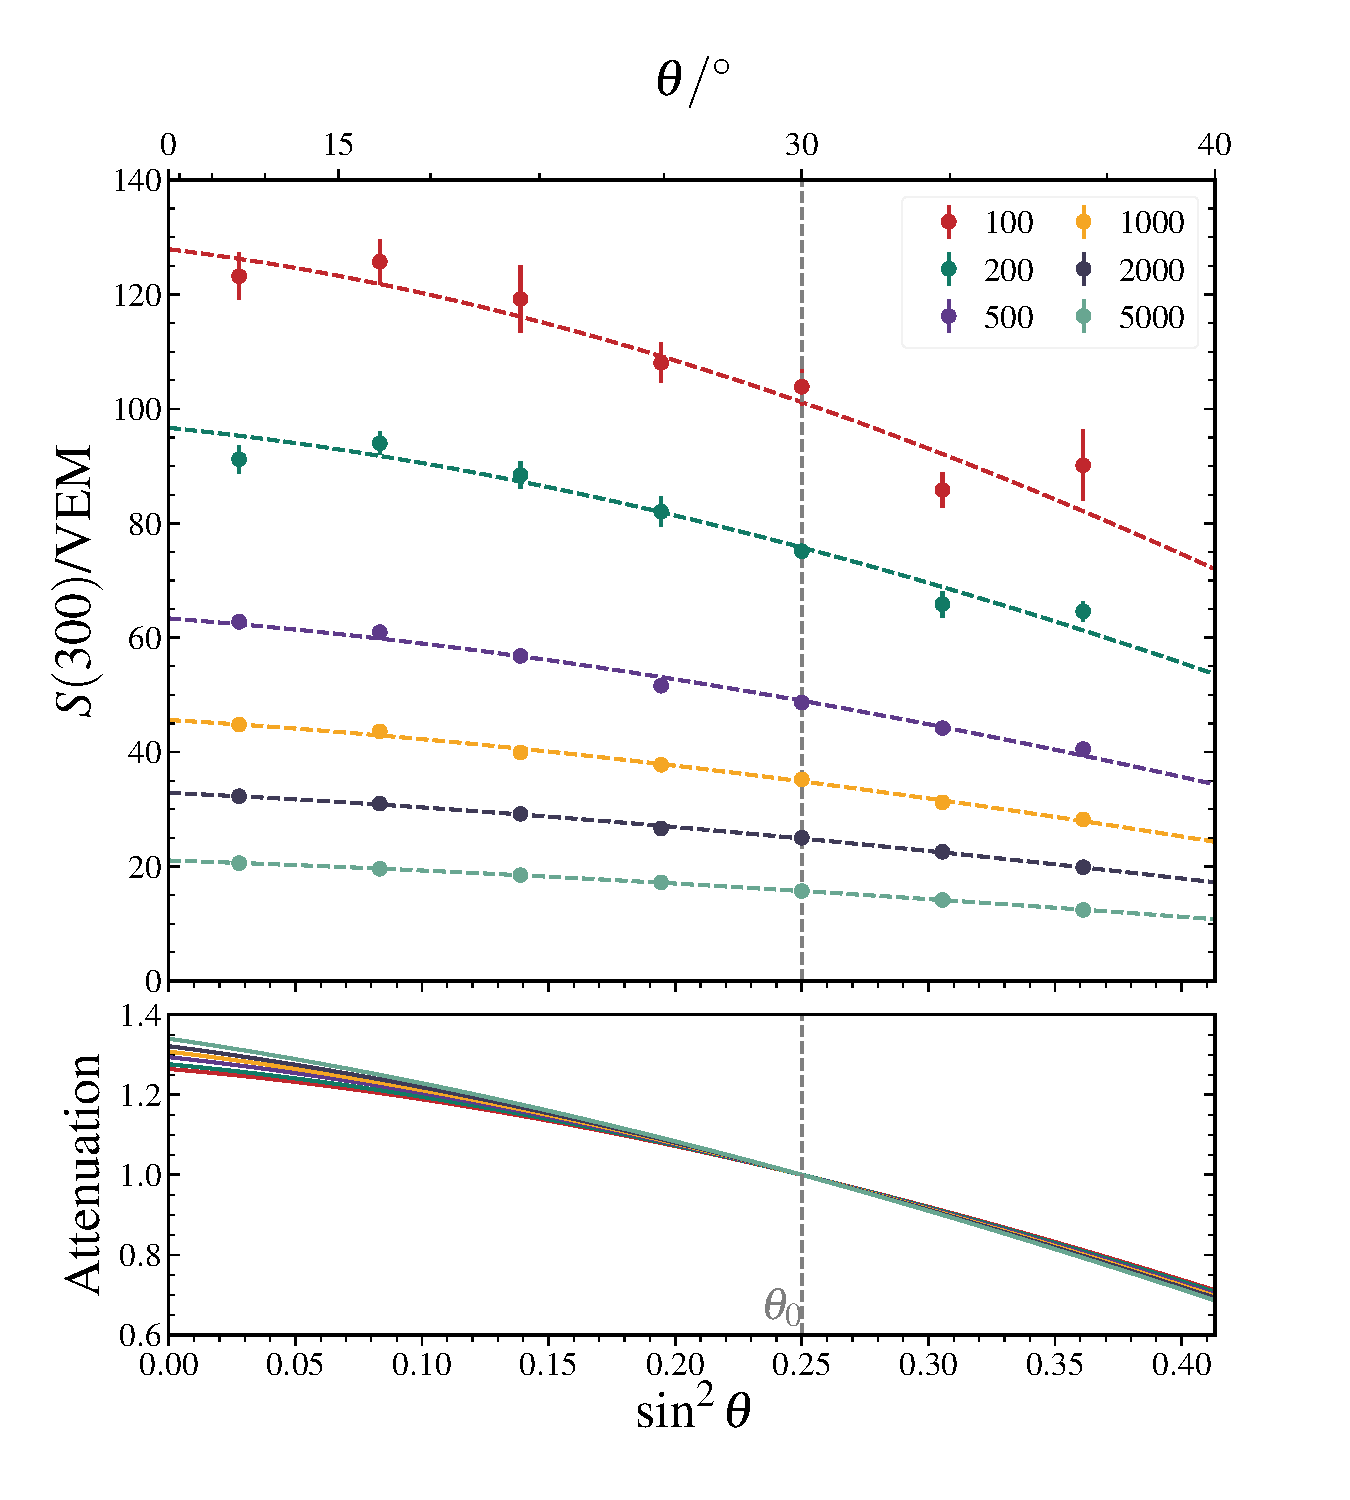
\includegraphics[width=0.85\textwidth]{figures/chapter_reconstruction/cic_global_fit.pdf}
    \caption{Global fit to the six constant-intensity cuts.
    The upper panel shows the values of $S(300)$ and the fitted curves, while the lower panel shows the corresponding attenuation functions.
    The vertical dashed line indicates the reference angle $\theta_{\text{ref}}=30^\circ$.}
    \label{fig:cic_global_fit}
\end{figure}

The effect of the CIC correction is shown in \cref{fig:cic_before_after}.
The upper panel shows the histogram of $S(300)$ in bins of zenith angle and shower size.
% The curve shows, for a fixed intensity, the decrease of the shower size towards larger zenith angles due to atmospheric attenuation.
After the correction, the corresponding distributions in $S_{30}$ become approximately independent of the zenith angle, as shown in the lower panel.
The solid and dashed lines indicate the approximate full-efficiency threshold before and after the correction, respectively.
Below this threshold, the distribution is distorted by the decreasing detection efficiency and should not be interpreted as a residual attenuation effect.
The corrected shower size $S_{30}$ is used as the estimator of the cosmic-ray energy.

\begin{figure}
    \centering
    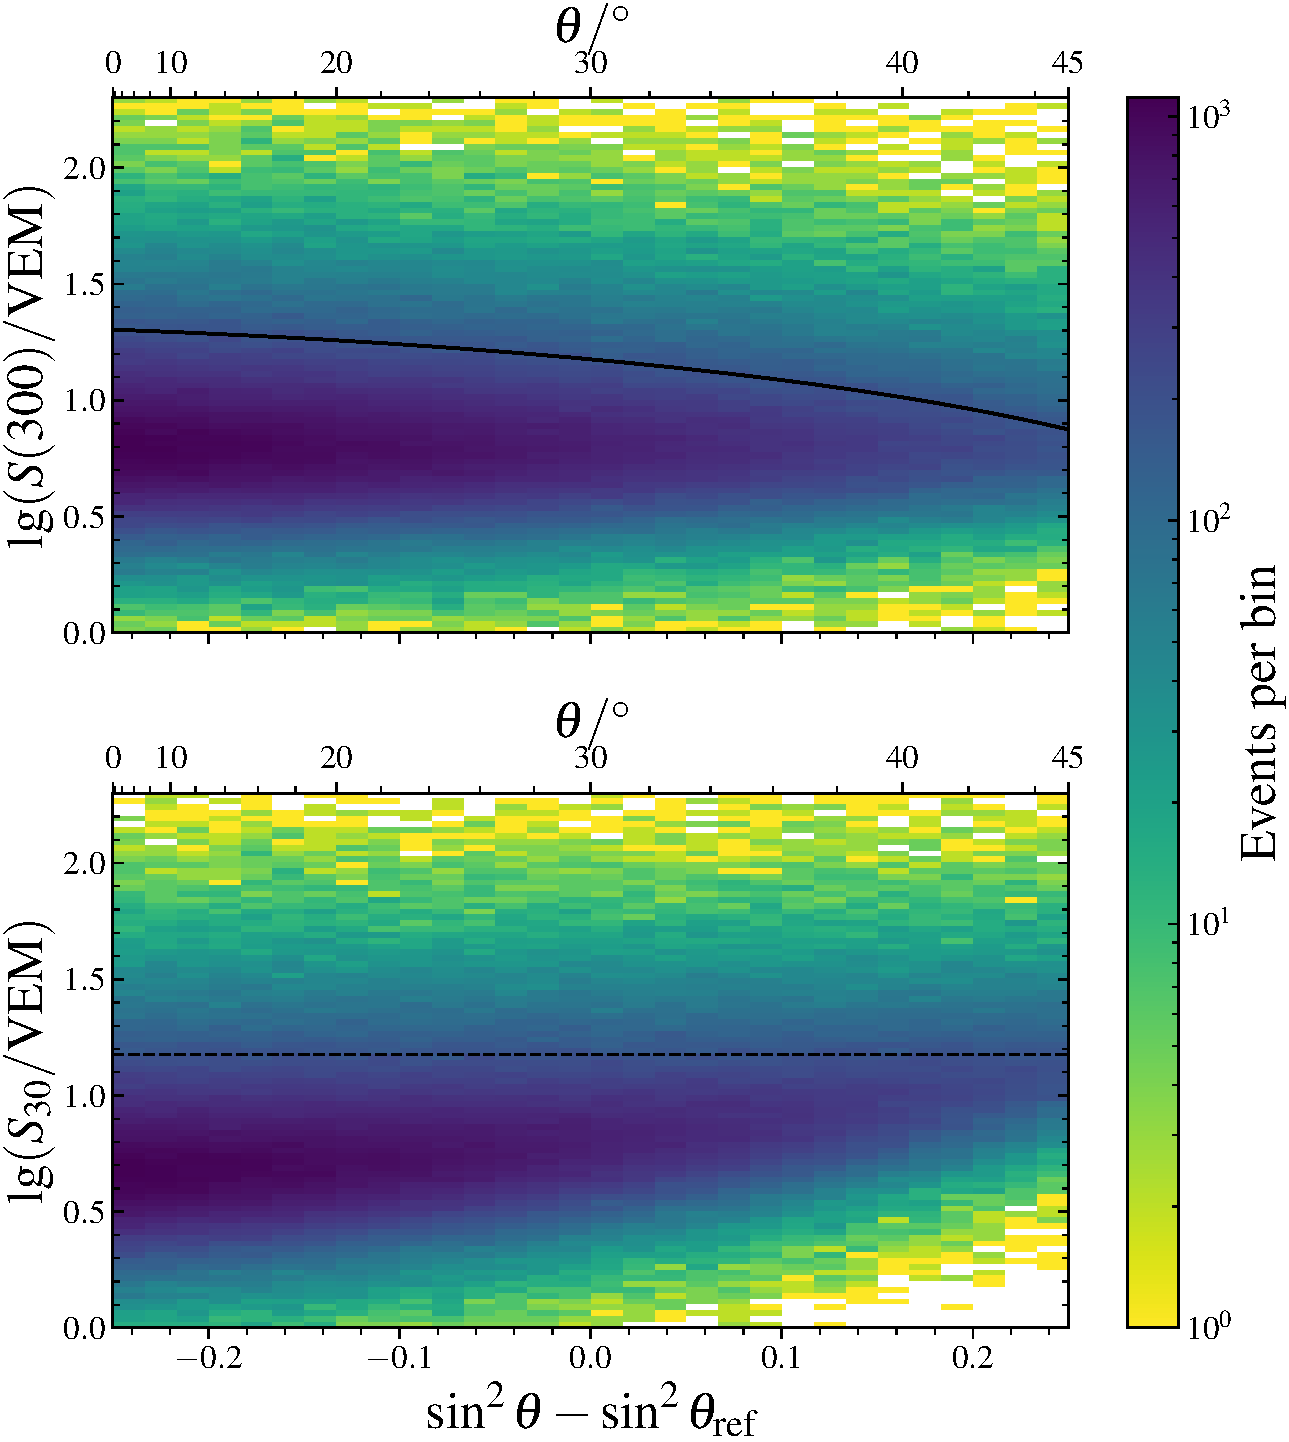
\includegraphics[width=0.85\textwidth]{figures/chapter_reconstruction/cic_before_after.pdf}
    \caption{Distribution of the shower size and zenith angle before and after the CIC correction.
    The solid line in the upper panel shows the attenuation curve corresponding to the full-efficiency threshold, $S_{30}=15\,\mathrm{VEM}$.
    The dashed line in the lower panel shows the same threshold after the conversion to $S_{30}$.}
    \label{fig:cic_before_after}
\end{figure}

\section{Energy calibration of the SD-433}
\label{sec:energy_calibration}
\label{sec:calibration}

With the attenuation in the atmosphere corrected, the shower size $S_{30}$ can be calibrated in terms of the primary energy.
The other two surface-detector arrays, the \sd{750} and \sd{1500}, are calibrated  using events detected simultaneously by the \gls{sd} and \gls{fd}.
However, because of the distance between the \sd{433} and the nearest \gls{fd} site, Cohihueco, the \gls{heat} telescopes cannot observe showers falling within the \sd{433} area.
The \sd{433} energy scale is therefore obtained through an \gls{sd}-\gls{sd} calibration using events detected in coincidence with the \sd{750}.
This introduces an additional complication because the \sd{750} calibration relation must be extrapolated by approximately two to three energy bins below the range in which that array is fully efficient, as discussed in \cref{sec:sd750_efficiency}.
The finite resolutions of both arrays, their correlation, and the event selection must consequently be included in the calibration fit.

\subsection{SD-750 reference scale and coincident events}
\label{subsec:calibration_sample}

The calibration requires events reconstructed with high quality by both arrays.
The standard spectrum-quality selections are therefore applied independently to the \sd{433} and \sd{750} datasets.
The events are required to have $\theta<40^\circ$, satisfy the 6T5 fiducial condition, and fall within periods of stable acquisition.
The \sd{750} dataset is obtained from an updated reconstruction of the data used in Ref.~\cite{PierreAuger:2021}, restricted to the same acquisition period as the \sd{433} dataset.
Its energies are recalculated using the updated ICRC 2025 calibration based on the revised \gls{fd} reconstruction~\cite{PierreAuger:2025:EnergyScale,2026:Verzi:CalibrationSD750}.

The \sd{750} energy calibration is described by the power law
\begin{align}
    E^{\text{SD-750}}
    =
    A^{\text{SD-750}}
    \left(
        \frac{S^{\text{SD-750}}_{35}}{S_0^{\text{SD-750}}}
    \right)^{B^{\text{SD-750}}},
    \label{eq:sd750_cal}
\end{align}
\noindent where $S^{\text{SD-750}}_{35}$ is the shower-size estimator corrected for atmospheric attenuation. 
The parameters $A^{\text{SD-750}}$ and  $B^{\text{SD-750}}$ respectively set the normalization and the slope of the calibration.
The values applied in this work are $A^{\text{SD-750}}=13.3\,\mathrm{PeV}$, $B^{\text{SD-750}}=1.00$, and $S_0^{\text{SD-750}}=1\,\mathrm{VEM}$.
% After recalibrating the \sd{750} events, the two datasets are matched by their event identifiers, yielding \num{37505} coincident events.

% TODO: Describe the SD-750 reference energy scale, the construction of the
% 37,505-event coincidence sample, the resolution model, and the S30 > 30 VEM
% calibration threshold that leaves 5,980 events for the fit.

\subsection{Likelihood fit and calibration relation}
\label{subsec:calibration_fit}

The relation between the \sd{433} shower size and the \sd{750} reference energy is also described by a power law,
\begin{align}
    E
    =
    A
    \left(
        \frac{S_{30}}{S_0}
    \right)^B,
    \label{eq:sd433_calibration}
\end{align}
where $S_0=40\,\mathrm{VEM}$ is chosen to be within the calibrated energy range to reduce the correlation between the normalization $A$ and the slope $B$.
The calibration is performed using the likelihood method introduced in~\cite{Dembinski:2016:Likelihood}.
The finite resolutions of both $S_{30}$ and the \sd{750} reference energy are included in the likelihood.
Unlike an \gls{sd}-\gls{fd} calibration, the two shower size and energy measurements are correlated because both arrays observe the same shower footprint and share some of the \gls{wcd}s.
For the \sd{750} resolution, the parameterization from Ref.~\cite{PierreAuger:2021} is adopted,
\begin{align}
    \frac{\sigma_{\mathrm{SD-750}}}{E}
    =
    \sqrt{
        \sigma_{\mathrm{sh}}^2
        +
        \left(\sigma_{\mathrm{det}}^{\mathrm{SD-750}}\right)^2
        \frac{E_0}{E}
    },
\end{align}
where $\sigma_{\mathrm{sh}}=0.09$ describes the energy-independent shower-to-shower fluctuations and $\sigma_{\mathrm{det}}^{\mathrm{SD-750}}=0.21$ parametrizes the detector contribution. A reference energy $E_0=100\,\mathrm{PeV}$ was chosen.

The $S_{30}$ resolution is estimated from \sd{750} assuming the same shower-to-shower fluctuations and detector contribution improved by a factor 3 given the increased detector density,
\begin{align}
    \frac{\sigma_{S_{30}}}{S_{30}}
    =
    \frac{1}{B_0}
    \sqrt{
        \sigma_{\mathrm{sh}}^2
        +
        \left(\sigma_{\mathrm{det}}^{\mathrm{SD-433}}\right)^2
        \frac{E_0}{E}
    },
\end{align}

where $\sigma_{\mathrm{det}}^{\mathrm{SD-433}}=0.12$. The factor $B_0$, reflecting the change from energy to shower size, was set to $1.0$ the value obtained from the calibration.  

Because both arrays sample the same shower, their shower-to-shower fluctuations are fully correlated.
An additional detector correlation arises from the \gls{wcd}s shared by the two arrays.
We consider these two contributions to model the correlation between the shower size measured by the \sd{433} and the energy measured by the \sd{750} with the approximated model, 

\begin{align}
    \rho
    =
    \frac{
        \displaystyle
        \frac{\sigma_{\mathrm{sh}}^2}{B_0}
        +
        \rho_{\mathrm{det}}
        \displaystyle
        \left(
            \frac{\sigma_{S}}{S_{30}}
        \right)
        \left(
            \frac{\sigma_{E}}{E^{\mathrm{SD-750}}}
        \right)
    }{
        \displaystyle
        \left(
            \frac{\sigma_{S}}{S_{30}}
        \right)
        \left(
            \frac{\sigma_{E}}{E^{\mathrm{SD-750}}}
        \right)
    },
\end{align}

where $\rho_{\mathrm{det}}=0.33$ is the fraction of \sd{433} detectors that are also in the \sd{750}.


For the $i$\-th event, the minimization performed to fit the calibration includes a quadratic term considering the resolutions of $S_{30}$ and $E^{\text{SD-750}}$ and their correlations,  

\begin{align}
    Q_i(s\mid A,B)
    =
    \frac{1}{1-\rho_i^2}
    \Bigg[
        &
        \left(
            \frac{S_{30,i}-s}{\sigma_{S,i}}
        \right)^2
        +
        \left(
            \frac{
                E_i^{\mathrm{SD-750}}
                -
                E_{\mathrm{cal}}(s\mid A,B)
            }{\sigma_{E,i}}
        \right)^2
        \nonumber\\
        &
        -
        2\rho_i
        \left(
            \frac{S_{30,i}-s}{\sigma_{S,i}}
        \right)
        \left(
            \frac{
                E_i^{\mathrm{SD-750}}
                -
                E_{\mathrm{cal}}(s\mid A,B)
            }{\sigma_{E,i}}
        \right)
    \Bigg].
    \label{eq:calibration_mahalanobis}
\end{align}

where an underlying shower size $s$ and the corresponding energy derived by the calibration model, $E_{\mathrm{cal}}(s\mid A,B)$ are scanned during the minimization procedure.  

The calibration parameters are fitted by maximizing the likelihood of the observed shower sizes and \sd{750} energies. For each event, the model considers a range of possible underlying shower sizes and the energy predicted for each by the calibration curve. A correlated Gaussian response describes the compatibility of the observed pair with each candidate, accounting for the uncertainties in both observables and their correlated fluctuations.

The likelihood averages these contributions using the measured size distribution as an empirical approximation to the underlying distribution. The candidate sizes are histogram bin centers, weighted by their relative frequencies. This accounts for the unequal abundance of showers of different sizes: several underlying sizes can produce the same observed pair, with different probabilities. The histogram includes events below the selection threshold, allowing those sizes to contribute to the likelihood of selected events through upward fluctuations. The fit combines the likelihoods of the selected events by summing their logarithms.
This follows the bootstrap approach in~\cite{Dembinski:2013:Unfolding}, adapted to use a histogram of shower sizes in place of a sample of energies.


The calibration of the \sd{750} was done with events with an energy measured by the FD above a given threshold. The other option, i.e. cutting on the shower size measured by the \sd{750}, was not applied as the FD has a better resolution than the \sd{750}. This criteria minimizes the fluctuations of sub-threshold events in the set of events selected for the calibration.
The opposite situation occurs in the \sd{433}, the calibrated detector has better resolution than the calibrator. Following the same principle of selection based on the the variable with better resolution, the event selection is applied to $S_{30}$ to minimize migration effects.

The cut $S_{30}>30\,\mathrm{VEM}$ roughly corresponds to the full-efficiency threshold of the \sd{750}, leaving \num{5980} available events for the calibration.
However, events below the cut are still indirectly used and account for migrations across the threshold.
The fit results in $A=(149.49\pm0.34)\,\mathrm{PeV}$ and $B=0.963\pm0.002$, with a correlation $\rho_{AB}=-0.51$.
The calibration threshold $S_{30}=30\,\mathrm{VEM}$ corresponds to an energy of $113.3\,\mathrm{PeV}$.

The systematic uncertainty associated with the choice of the calibration threshold is evaluated by repeating the fit for $S_{30,\min}$ between $15$ and $40\,\mathrm{VEM}$.
As the threshold increases, the normalization $A$ decreases while the slope $B$ increases.
The full excursion of the fitted parameters is assigned as the systematic uncertainty, yielding $\Delta A_{\mathrm{syst}}=4.0\,\mathrm{PeV}$ and $\Delta B_{\mathrm{syst}}=0.035$.
The fit with $S_{30,\min}=15\,\mathrm{VEM}$, the minimum limit under consideration, extends well below the nominal \sd{750} efficiency range and approximately down to the full-efficiency threshold of the \sd{433}, therefore providing a conservative estimate of the systematic envelope.

\begin{figure}
    \centering
    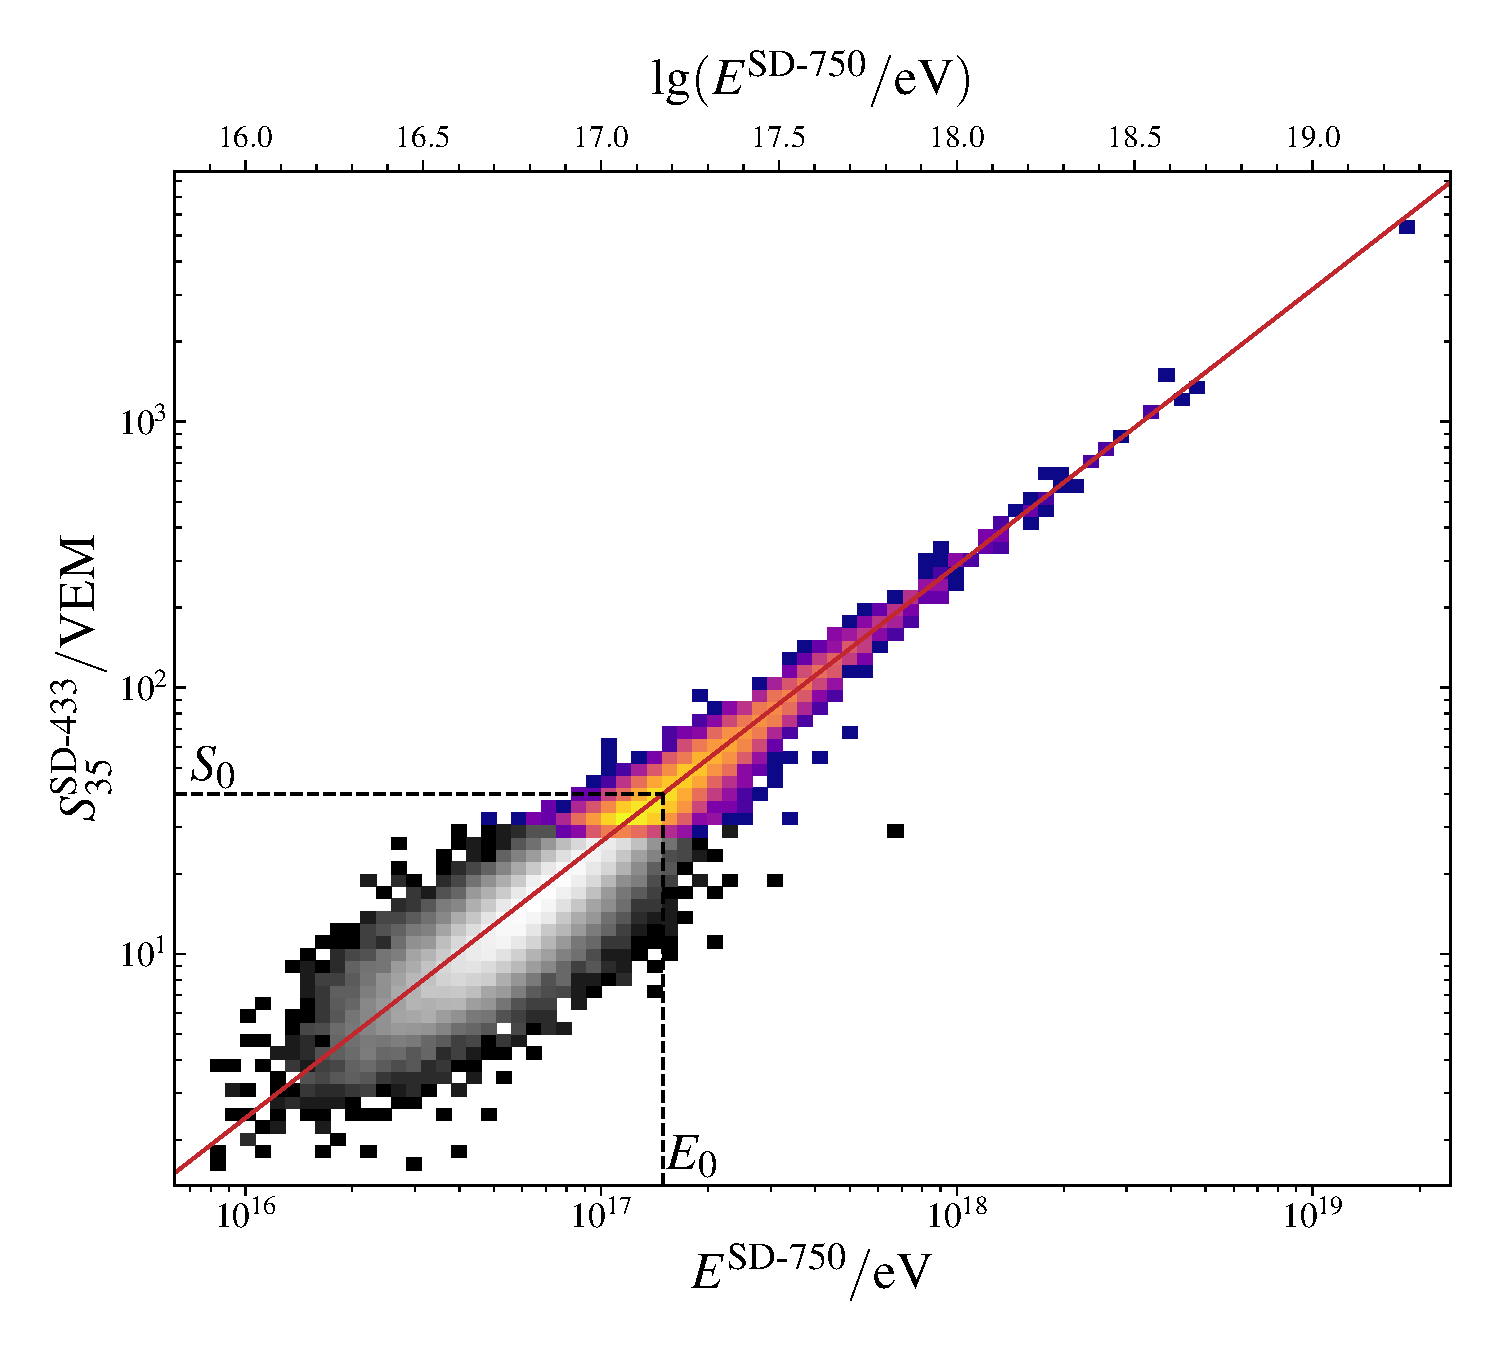
\includegraphics[width=0.85\textwidth]{figures/chapter_reconstruction/energy_calibration.pdf}
    \caption{Calibration of the \sd{433} shower size $S_{30}$ against the \sd{750}  energy using coincident events. The color scale shows the event density above the calibration threshold, while events below the threshold are shown in gray. The red line shows the fitted calibration relation. The dashed lines indicate the normalization point $S_0=40\,\mathrm{VEM}$ and its corresponding energy.}
    \label{fig:sd433_energy_calibration}
\end{figure}

% \subsection{Calibration residuals and application}
% \label{subsec:calibration_validation}

% TODO: Discuss the calibration residuals, the 113.3 PeV energy associated
% with the 30 VEM calibration cut, and application of the relation to the
% 382,131-event SD-433 dataset used for the spectrum measurement.

The relative difference between the \sd{750} energy and the calibrated \sd{433} energy is shown in the left panel of \cref{fig:sd433_energy_calibration_residuals}.
The points correspond to individual events.
Events below the $S_{30,\min}=30\,\mathrm{VEM}$ shower-size threshold are shown in gray, while the events used for the \sd{433} calibration are shown in green.
The red points show the mean residual in bins of width $\Delta\lg(E^{\mathrm{SD-433}}/\mathrm{eV})=0.1$ below $\lg(E^{\mathrm{SD-433}}/\mathrm{eV})=18$ and $0.3$ above to increase the statistics.
The error bars indicate the standard error of the mean.
Although individual residuals can reach approximately $20\%$, the mean residual remains close to zero and decreases rapidly with energy.
The positive residual below the threshold is produced by migration across the event selection and is not included in the fit.

Finally, the energy distribution of the \sd{433} events is shown in the right panel of \cref{fig:sd433_energy_calibration_residuals}, together with the full-efficiency threshold.
Below this threshold, the detection efficiency increases with energy, producing the rising event distribution despite the decreasing cosmic ray flux.
Above full efficiency, the distribution decreases approximately linearly on the logarithmic scale, as expected for a power-law-like spectrum.
This distribution forms the basis for the raw spectrum determined in \cref{sec:raw_spectrum} and the subsequent characterization of the second knee.

\begin{figure}
    \centering
    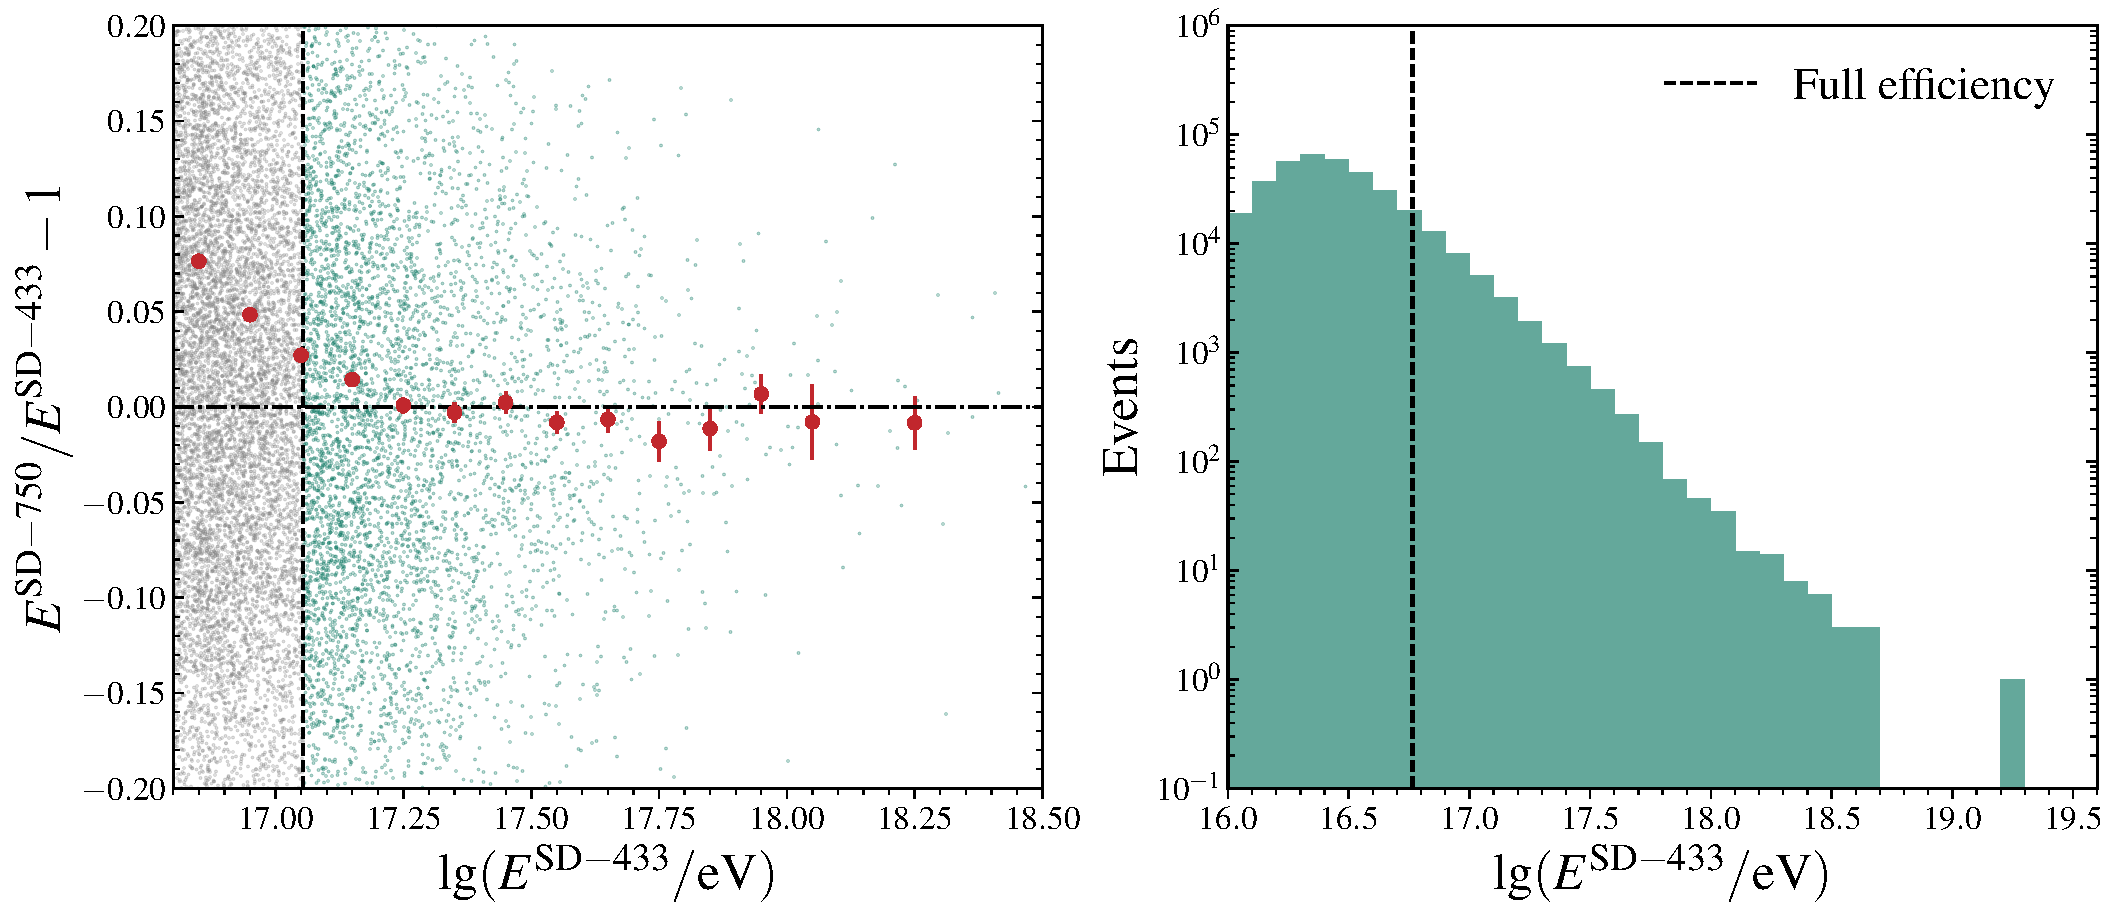
\includegraphics[width=\textwidth]{figures/chapter_reconstruction/energy_calibration_residuals.pdf}
    \caption{Left: relative difference between the \sd{750} reference energy and the calibrated \sd{433} energy. The points show individual events and the red markers show the mean residual in energy bins, with error bars indicating the uncertainty of the mean. Right: energy distribution of the full \sd{433} dataset. The dashed line indicates the full-efficiency energy.}
    \label{fig:sd433_energy_calibration_residuals}
\end{figure}

\section{Energy resolution and bias}
\label{sec:res_and_bias}

The energy resolution and bias enter the detector response used to fit and unfold the cosmic-ray spectrum measured with the \sd{433}.
Their parameterizations are obtained from the same simulations used to determine the detection efficiency in \cref{sec:efficiency}, adopting the mixed composition inferred from the \gls{gsf} model~\cite{Rodriguez:2026:Thesis}.
The denser spacing of the \sd{433} provides more triggered stations at a given energy, better constraining the shower-size reconstruction and yielding a better energy resolution than that of the \sd{750}.
Comparisons using events reconstructed jointly by the two arrays provide a consistency check of the \sd{433} shower size and \sd{750} resolutions modeled for the calibration.

In addition, the bias of the \sd{433} energy is determined by comparing the simulated and reconstructed energies, $E_{\mathrm{rec}}/E_{\mathrm{MC}}-1$.
These residuals are evaluated using the simulation-based calibration, while the energy dependence is expressed in terms of the true energy mapped onto the \sd{433} data scale, denoted here by $E$.
The bias is parameterized as
\begin{align}
    b(E)
    &= b_0\exp\!\left[-b_1\left(\lg(E/\mathrm{eV})-16\right)\right]+b_2,
    \label{eq:energy_bias}
\end{align}
with
\begin{align}
    b_0 &= 0.30 \pm 0.01, &
    b_1 &= 10.0 \pm 0.3, &
    b_2 &= 0.005 \pm 0.001.
\end{align}
Below full efficiency, upward fluctuations are preferentially selected, producing a positive bias that increases towards lower energies.
Above the full-efficiency threshold, this contribution becomes small.

The relative energy resolution is described by the quadratic sum of a constant contribution from shower-to-shower fluctuations and an energy-dependent detector contribution,
\begin{align}
    \frac{\sigma(E)}{E}
    &= \sqrt{R_{\mathrm{sh}}^2
       +\frac{R_0^2}{E/(10^{17}\,\mathrm{eV})}},
    \label{eq:resolution_sigma}
\end{align}
where the fit to the simulated \gls{gsf} mixture yields
\begin{align}
    R_{\mathrm{sh}} &= 0.103 \pm 0.001, &
    R_0 &= 0.096 \pm 0.005.
\end{align}
The detector contribution decreases with increasing energy, and the relative resolution approaches the shower-fluctuation limit of approximately $10.3\%$. 
The resolution derived from simulations is consistent with the model used in the calibration.
% Here, $\sigma(E)$ denotes the absolute energy resolution used in the response function for the spectrum analysis.
The bias and relative resolution parameterizations are shown in \cref{fig:sd433_res_bias}.


\begin{figure}
    \centering
    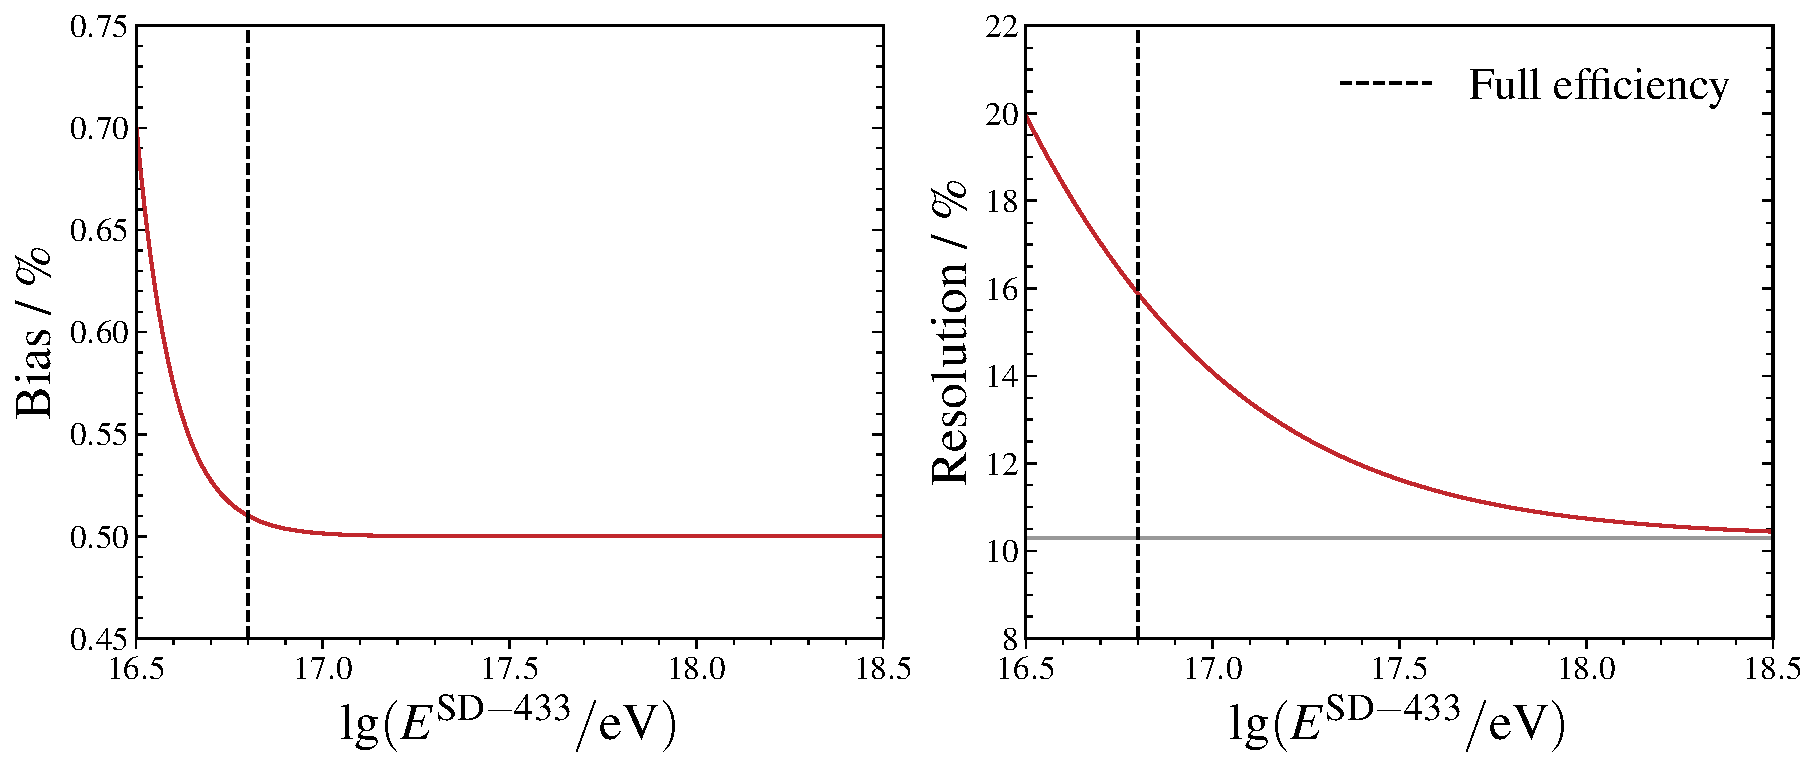
\includegraphics[width=\textwidth]{figures/chapter_reconstruction/sd433_resolution_bias.pdf}
    \caption{Energy bias (left) and resolution (right) parameterizations obtained from simulations using the GSF mixed composition. The dashed lines indicate the full-efficiency threshold. Adapted from Ref.~\cite{Rodriguez:2026:Thesis}.}
    \label{fig:sd433_res_bias}
\end{figure}

\section{Summary}
\label{sec:energy_reconstruction_summary}

In this chapter we presented the energy reconstruction of the events recorded with the \sd{433}.
After reconstructing the shower geometry, the shower size $S(300)$ is obtained by modeling the decrease of the signal with the distance to the shower core.
From the reconstructed $S(300)$, the attenuation function is determined to correct for the different zenith angles of the showers.
The zenith-independent shower size $S_{30}$ is then obtained by iteratively applying the shower-size-dependent correction $f_{\mathrm{CIC}}(\theta,S_{30})$.
Using the events detected in common with the \sd{750} we then developed the energy calibration for the \sd{433}.
The likelihood formalism was introduced to take into account the finite resolution both of \sd{433} shower size and the \sd{750} energy.
An empirical shower-size distribution is included to account for the preferential migration from low to high energies produced by the steep cosmic ray spectrum.
Minimizing the log-likelihood yields the calibration parameters $A=(149.49\pm0.34)\,\mathrm{PeV}$ and $B=0.963\pm0.002$.
The mean difference between the calibrated \sd{433} energy and the \sd{750} reference energy remains below $3\%$ throughout the fitted energy range and decreases with increasing energy.
Finally, the calibrated \sd{433} energy forms the basis of the cosmic ray spectrum measurement presented in the next chapter.
% TODO: Summarize the continuous reconstruction chain from the Offline
% determination of S(300), through the CIC correction to S30, to the calibrated
% SD-433 energy used in the spectrum measurement.

\end{document}
